\documentclass{article}
\usepackage{tikz}
\usepackage{xcolor}

\definecolor{myblue}{RGB}{40,110,160}
\definecolor{bggray}{RGB}{240,240,240}
\definecolor{gridgray}{RGB}{180,180,180}

\begin{document}

\begin{center}
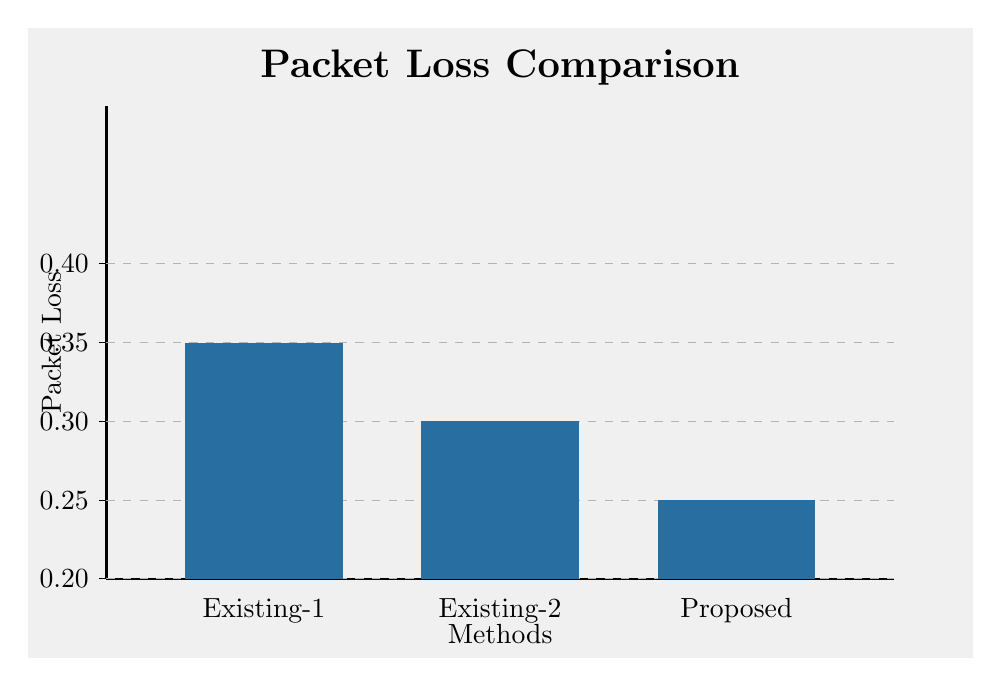
\begin{tikzpicture}

% Background
\fill[bggray] (0,0) rectangle (12,8);

% Axes
\draw[thick] (1,1) -- (1,7); % Y-axis
\draw[thick] (1,1) -- (11,1); % X-axis

% Title
\node[font=\Large\bfseries] at (6,7.5) {Packet Loss Comparison};

% Labels
\node[rotate=90] at (0.3,4) {Packet Loss};
\node at (6,0.3) {Methods};

% Y-axis ticks + grid lines
\foreach \y/\val in {
1/0.20,2/0.25,3/0.30,4/0.35,5/0.40
} {
    \draw (0.9,\y) -- (1.1,\y);
    \node[left] at (0.9,\y) {\val};

    % Grid lines
    \draw[dashed, gridgray] (1,\y) -- (11,\y);
}

% Bars (scaled from 0.20–0.40)
\def\scale{20}

\fill[myblue] (2,1) rectangle (4,{1 + (0.35-0.20)*\scale});
\fill[myblue] (5,1) rectangle (7,{1 + (0.30-0.20)*\scale});
\fill[myblue] (8,1) rectangle (10,{1 + (0.25-0.20)*\scale});

% X labels
\node at (3,0.6) {Existing-1};
\node at (6,0.6) {Existing-2};
\node at (9,0.6) {Proposed};

\end{tikzpicture}
\end{center}

\end{document}